\documentclass[11pt,a4paper]{article}
\usepackage{amsmath}
\usepackage{amsthm}
\usepackage{amssymb}
\usepackage{booktabs}
\usepackage{graphicx}
\usepackage{color}
\usepackage{fullpage}
\usepackage{listings}
\usepackage{color}
\usepackage{url}
\usepackage{multirow}
\usepackage{forest}
% 為了讓表格緊密
\usepackage{float}
% 為了首行空格
%\usepackage{indentfirst}
% % 為表格添加 footnote
% \usepackage{tablefootnote}

\usepackage{tabularx}

% 全域格式設定（放在 preamble）
\lstset{
  numbers=left,
  numberstyle=\tiny\color{gray},
  stepnumber=1,
  numbersep=5pt,
  frame=single,
  basicstyle=\ttfamily\small,
  breaklines=true,
  showspaces=false,        % ← 明確關掉，確保空格不顯示為 ␣
  showstringspaces=false   % ← 字串內的空格也不顯示為 ␣
}

% 語言定義只放語言相關設定
\lstdefinelanguage{JavaScript}{
  keywords={break, case, ...},
  morekeywords=[2]{class, const, ...},
  sensitive=true,
  morecomment=[l]{//},
  morecomment=[s]{/*}{*/},
  morestring=[b]',
  morestring=[b]"
}

\lstdefinelanguage{Bash}{
  keywords={cd, npm, npx, ...},
  sensitive=true,
  morestring=[b]',
  morestring=[b]"
}

%yaml
\lstdefinelanguage{YAML}{
  keywords={name, on, jobs, steps, uses, with, run, ...},
  sensitive=true,
  morestring=[b]',
  morestring=[b]"
}

% for Chinese
\usepackage{fontspec} % 加這個就可以設定字體
\usepackage[BoldFont, SlantFont]{xeCJK} % 讓中英文字體分開設置
\setCJKmainfont{Microsoft JhengHei}  % 設定中文為系統上的字型，而英文不去更動，使用原TeX字型
\setCJKmonofont{Microsoft JhengHei} % 定義 CJK 等寬字型，避免 xeCJK 無法識別 \CJKttdefault
\renewcommand{\baselinestretch}{1.3}

\parskip=5pt
\parindent=24pt
\newtheorem{lemma}{Lemma}
\newtheorem{ques}{Question}
\newtheorem{prop}{Proposition}
\newtheorem{defn}{Definition}
\newtheorem{rmk}{Remark}
\newtheorem{note}{Note}
\newtheorem{eg}{Example}
\newtheorem{aspt}{Assumption}

\definecolor{emphOrange}{RGB}{247, 80, 0}
\definecolor{stringGray}{RGB}{109, 109, 109}
\definecolor{commentGreen}{RGB}{0, 96, 0}
\definecolor{mygreen}{rgb}{0,0.6,0}
\definecolor{mygray}{rgb}{0.5,0.5,0.5}
\definecolor{mymauve}{rgb}{0.58,0,0.82}



% "摘要", "表", "圖", "參考文獻"
\renewcommand{\abstractname}{\bf 摘要}
\renewcommand{\tablename}{表}
\renewcommand{\figurename}{圖}
\renewcommand{\refname}{\bf 參考文獻}

% -----
% 我在這裡加入了 tikz 和 forest 宏包 (基於 tikz) 來繪製 B+ Tree
\usepackage{tikz} % <<< --- 新增：明確載入 tikz
\usepackage{forest}
\usetikzlibrary{arrows.meta, chains}
% -----


\begin{document}

\title{雲原生 HW4 - CI/CD Pipeline}
\author{資管三 B12705041 李倢安}
\date{\today}
\maketitle
%\fontsize{20}{20pt}\selectfont
My GitHub Repository: \url{https://github.com/LEE-CHIEN-AN/cicd-lab}

\section*{CI Pipeline 說明}

本次作業為 \texttt{cicd-lab} 專案建立一條完整的 CI Pipeline，
檔案路徑為 \path{.github/workflows/ci_b12705041.yaml}，完整內容如下：
\begin{lstlisting}[language=YAML]
name: CI b12705041

on:
  push:
    branches:
      - '**'
  pull_request:

permissions:
  contents: read
  checks: write

jobs:
  ci:
    runs-on: ubuntu-latest

    steps:
      - name: Checkout
        uses: actions/checkout@v5

      - name: Setup Node.js
        uses: actions/setup-node@v5
        with:
          node-version: '22'
          cache: npm

      - name: Install dependencies
        run: npm ci

      - name: TypeScript typecheck
        run: npm run typecheck

      - name: Prettier check
        run: npm run format:check

      - name: Lint
        run: npm run lint

      - name: Run tests
        run: |
          mkdir -p reports
          npm test -- --reporter=default --reporter=junit \
            --outputFile.junit=reports/vitest-junit.xml

      - name: Publish test results
        uses: dorny/test-reporter@v1
        if: always()
        with:
          name: Vitest Test Results
          path: reports/vitest-junit.xml
          reporter: java-junit
\end{lstlisting}

\subsection*{Pipeline 設計說明}

\textbf{觸發條件（\texttt{on}）}

Pipeline 設定在兩種情境下自動執行：
\begin{itemize}
    \item \texttt{push}（任意 branch）：開發者每次推送程式碼，立即觸發品質檢查，確保問題在早期被發現。
    \item \texttt{pull\_request}：開 PR 時自動觸發，在合併進 \texttt{main} 之前強制通過所有檢查，保護主線品質。
\end{itemize}

\textbf{權限設定（\texttt{permissions}）}

\begin{itemize}
    \item \texttt{contents: read}：允許 Workflow 讀取 Repository 內容，\texttt{actions/checkout} 需要此權限。
    \item \texttt{checks: write}：允許 \texttt{dorny/test-reporter} 將測試結果寫入 GitHub Checks 系統，使測試報告直接顯示於 Actions 頁面，而不只是可下載的 Artifact。
\end{itemize}

\textbf{執行環境（\texttt{runs-on}）}

使用 \texttt{ubuntu-latest}，即 GitHub 提供的全新 Ubuntu 虛擬機。每次觸發都從乾淨環境開始，避免前次執行的殘留干擾，執行結束後自動刪除。

\textbf{步驟說明（\texttt{steps}）}

Pipeline 共分為七個步驟，設計原則為「越快速的靜態檢查越優先，越耗時的動態測試越靠後」，一旦前面的步驟失敗即立即中止，避免浪費運算資源：

\begin{enumerate}
    \item \textbf{Checkout}：使用 \texttt{actions/checkout@v5} 將 Repository 程式碼下載至 Runner VM，是幾乎所有 Workflow 的第一步。

    \item \textbf{Setup Node.js}：使用 \texttt{actions/setup-node@v5} 安裝指定版本 Node.js（v22）。啟用 \texttt{cache: npm}，將 \texttt{node\_modules} 快取，若 \texttt{package-lock.json} 未變動則直接使用快取，可省去 15--30 秒的下載時間。

    \item \textbf{Install dependencies}：執行 \texttt{npm ci}，嚴格依照 \texttt{package-lock.json} 安裝套件，確保 CI 環境與本機環境版本完全一致，避免「本機可以跑但 CI 失敗」的問題。

    \item \textbf{TypeScript typecheck}：執行 \texttt{npm run typecheck}，實際呼叫 \texttt{tsc --noEmit}，以 TypeScript 編譯器進行純型別檢查而不輸出檔案。TypeScript 型別錯誤在 Runtime 不會立即顯現，CI 在合併前提早捕捉，降低生產環境出現隱性 Bug 的風險。

    \item \textbf{Prettier check}：執行 \texttt{npm run format:check}，實際呼叫 \texttt{prettier --check .}，依照 \texttt{.prettierrc} 規定檢查所有檔案的格式（縮排、引號、分號等）。此步驟只做檢查，不自動修正；格式不符即直接失敗，強制團隊維持統一的程式碼風格。

    \item \textbf{Lint}：執行 \texttt{npm run lint}，使用 ESLint 搭配 \texttt{@typescript-eslint} 插件進行靜態程式碼分析，偵測潛在的程式邏輯錯誤與不良實踐。\texttt{actions/setup-node} 會自動載入 ESLint 的 Problem Matcher，讓 ESLint 錯誤直接標注在 PR 的程式碼行數上。

    \item \textbf{Run tests}：執行 \texttt{npm test}，以 Vitest 框架運行所有測試。同時使用兩種 Reporter：\texttt{default} 將結果輸出至 Log，\texttt{junit} 將結果輸出為 JUnit XML 格式（\texttt{reports/vitest-junit.xml}），供下一步解析。

    \item \textbf{Publish test results}：使用 \texttt{dorny/test-reporter@v1} 讀取 JUnit XML，將測試結果以圖形化方式呈現於 GitHub Actions 頁面的 Checks 區塊，可直接看到每個測試案例的通過或失敗狀態。設定 \texttt{if: always()} 確保即使測試步驟失敗，報告仍會被發布，讓開發者能立即得知是哪個測試壞掉。
\end{enumerate}

\section*{CI 執行結果截圖}

以下為 CI Pipeline 成功執行的截圖。最新一次的 \path{.github/workflows/ci_b12705041.yaml} 執行所有步驟均通過，Checks 區塊顯示 Vitest 測試結果，2 個測試案例全數通過。

\begin{figure}[H]
    \centering
    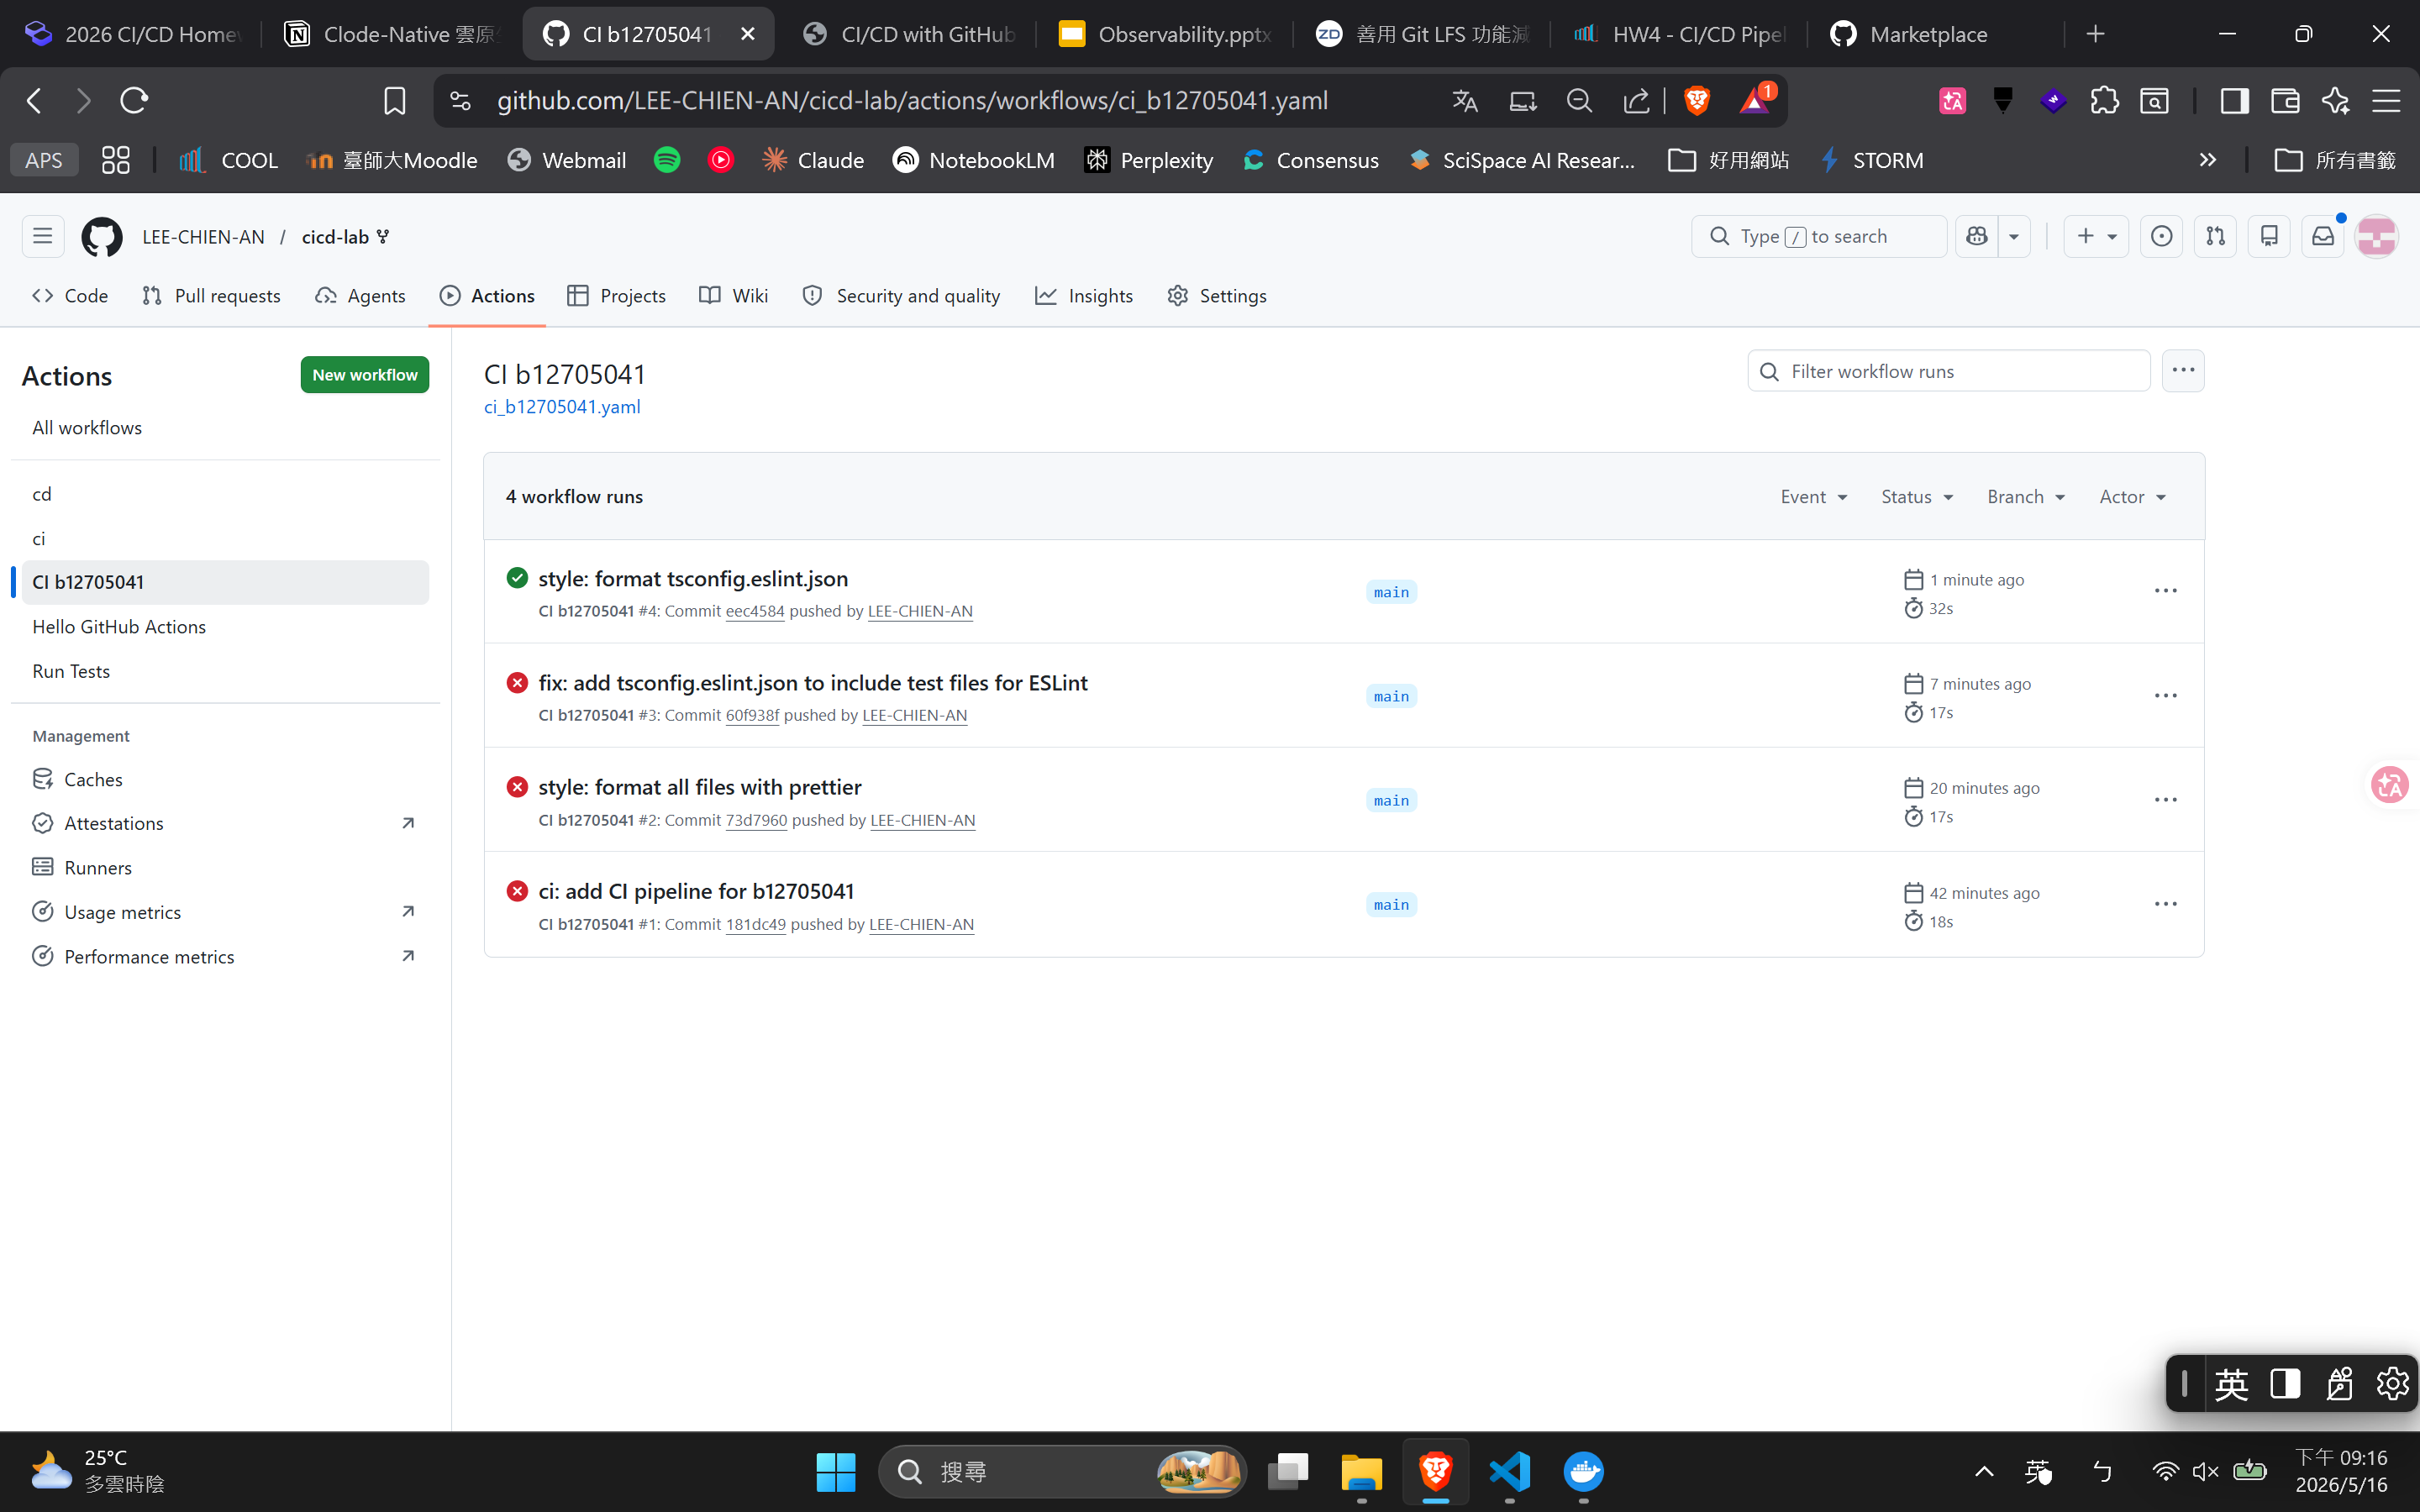
\includegraphics[width=0.8\textwidth]{image5.png}
    \caption{GitHub Actions 頁面顯示最新一次的測試所有 Steps 成功通過}
\end{figure}
\begin{figure}[H]
    \centering
    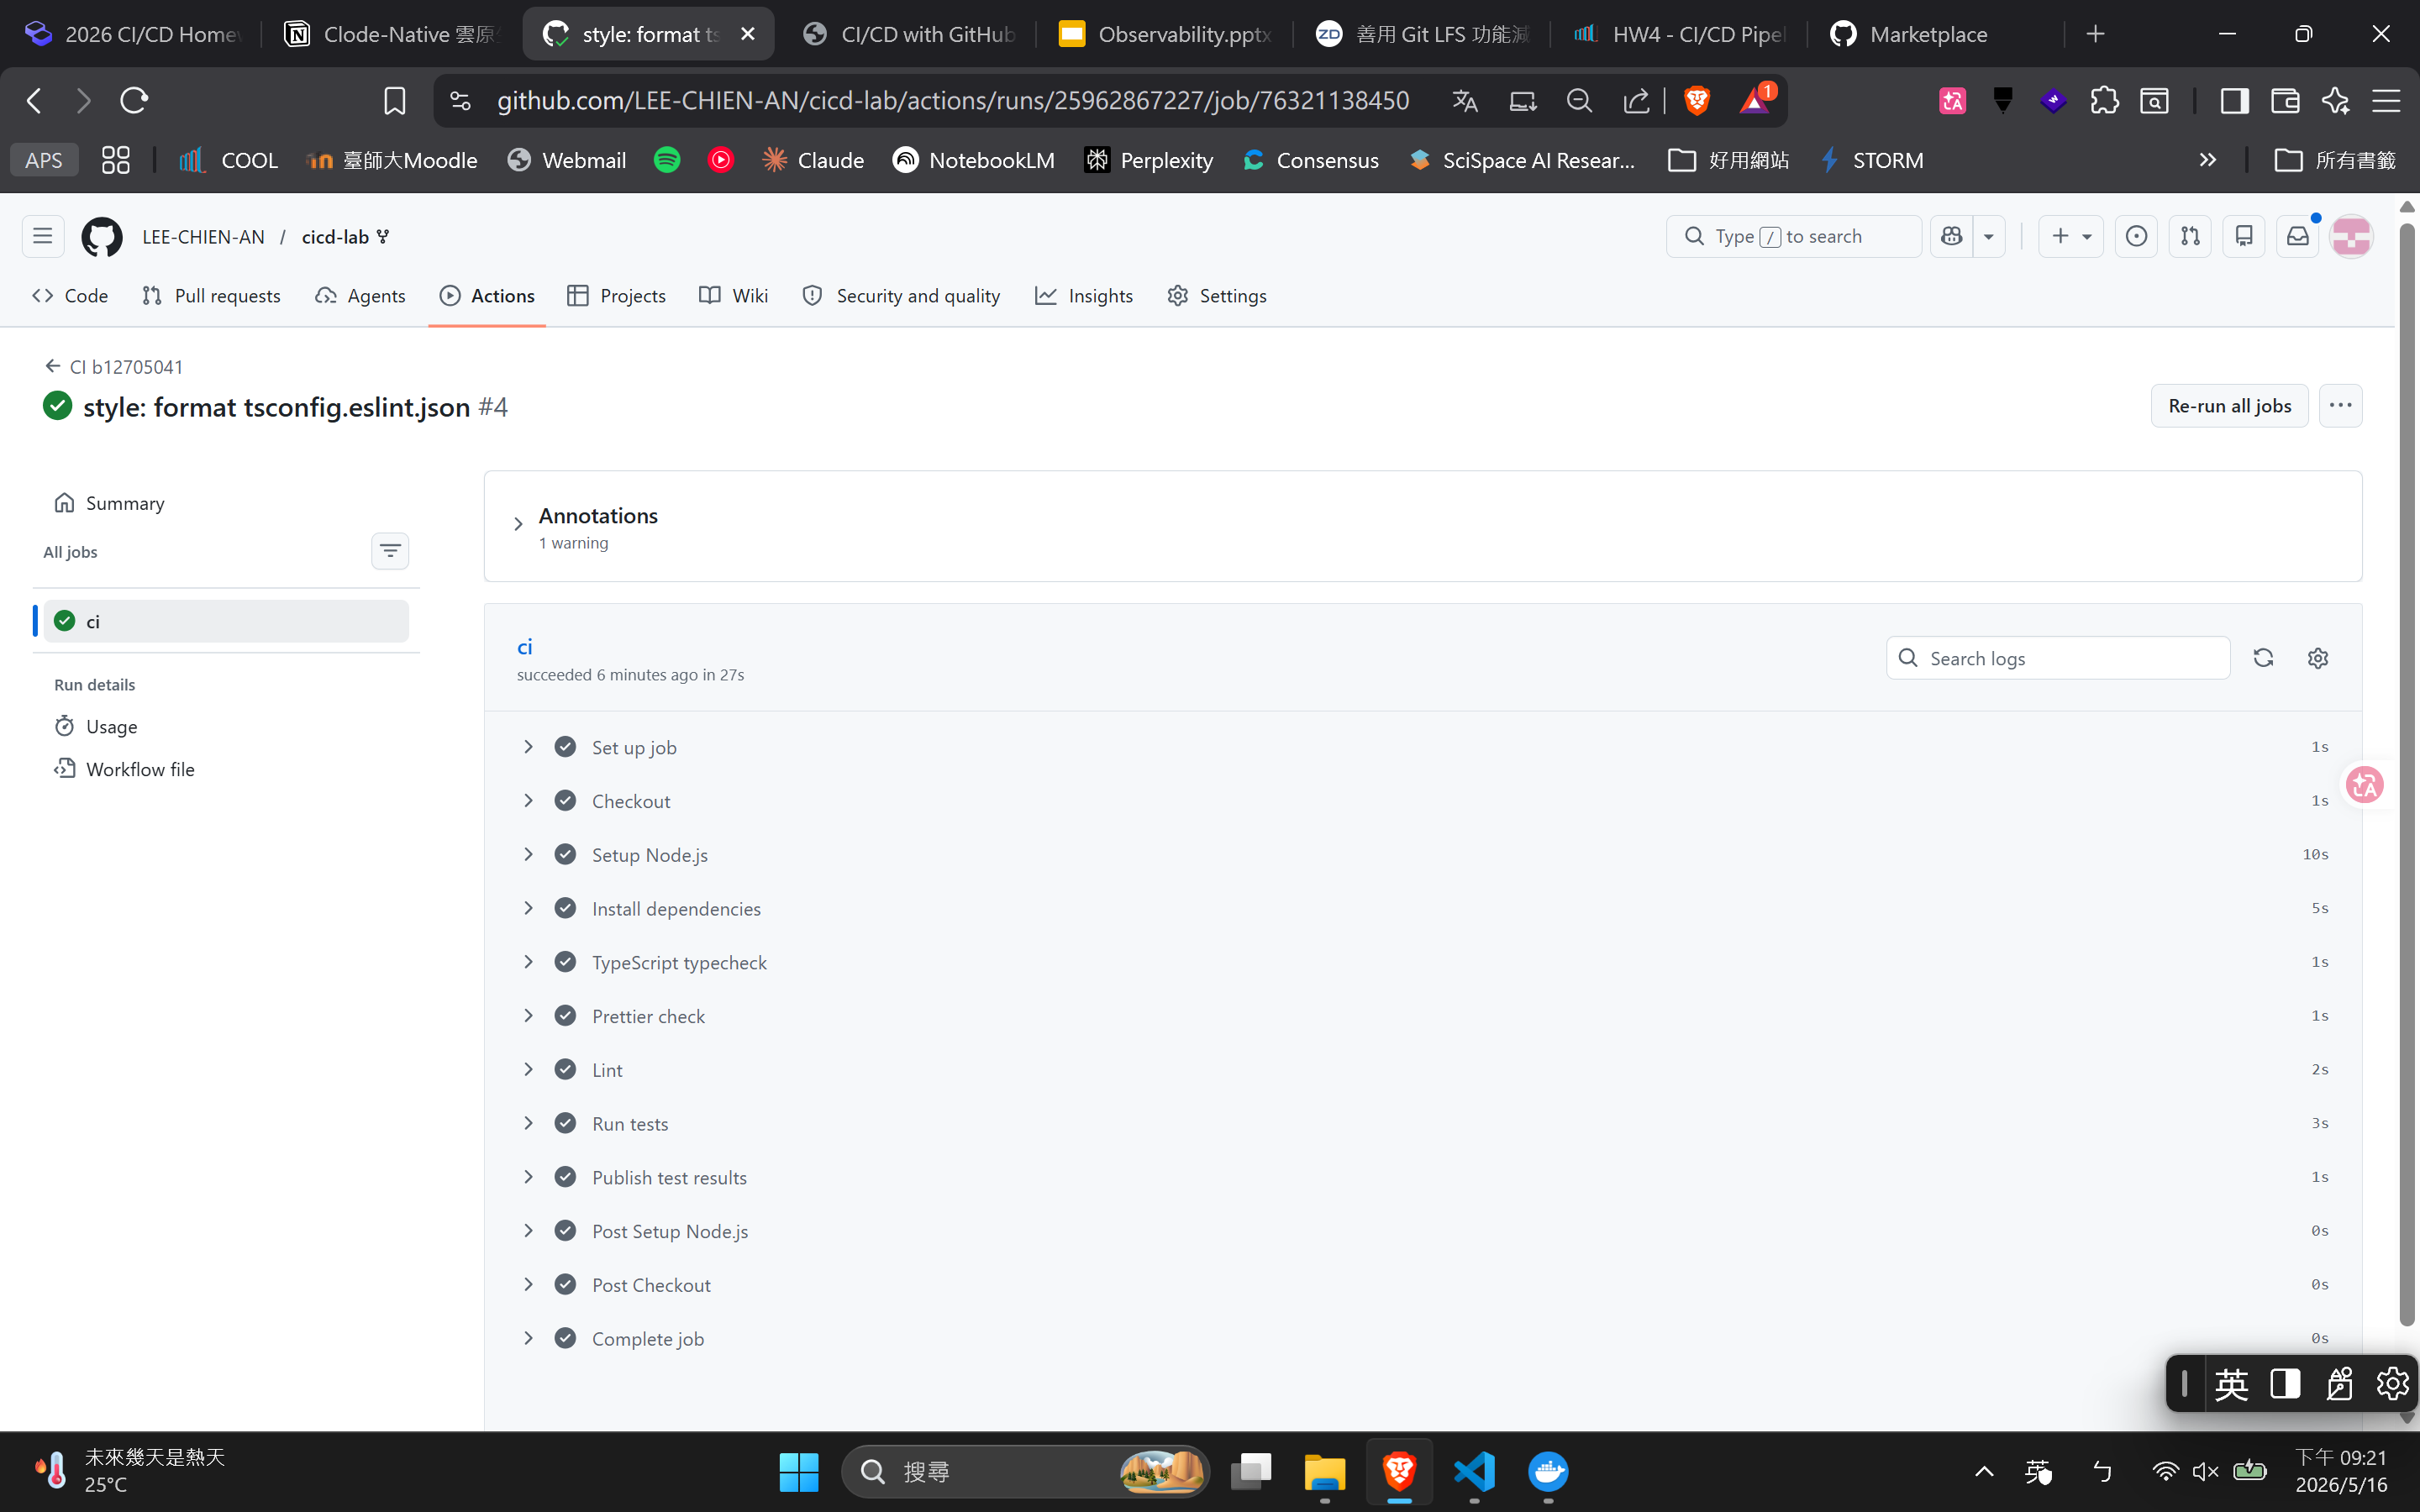
\includegraphics[width=0.8\textwidth]{image6.png}
    \caption{Checks 頁面顯示 Vitest Test Results 詳細測試報告}
\end{figure}

\section*{失敗案例說明}

在開發過程中共遭遇兩個導致 Pipeline 失敗的問題，以下分別說明其原因與修復方式。

\subsection*{案例一：Prettier 格式檢查失敗}

\textbf{錯誤原因}

新增 Workflow 檔案後，這些 YAML 檔案的縮排與格式未符合 \texttt{.prettierrc} 的規定，CI 執行至 \texttt{Prettier check} 步驟時立即失敗：

\begin{lstlisting}
[warn] .github/workflows/ci_b12705041.yaml
[warn] .github/workflows/01_hello.yaml
[warn] docker-compose.yml
Code style issues found in 7 files. -> exit code 1
\end{lstlisting}

\textbf{連鎖反應}

由於 Pipeline 在 Prettier 步驟中斷，後續的 \texttt{Lint}、\texttt{Run tests} 步驟均未執行，導致測試報告檔案（\texttt{reports/vitest-junit.xml}）從未被產生。\texttt{dorny/test-reporter} 雖因 \texttt{if: always()} 仍會執行，但找不到報告檔案，因而出現「No test report files were found」的第二個錯誤。此錯誤是 Prettier 失敗的連鎖結果，而非獨立問題。

\begin{figure}[H]
    \centering
    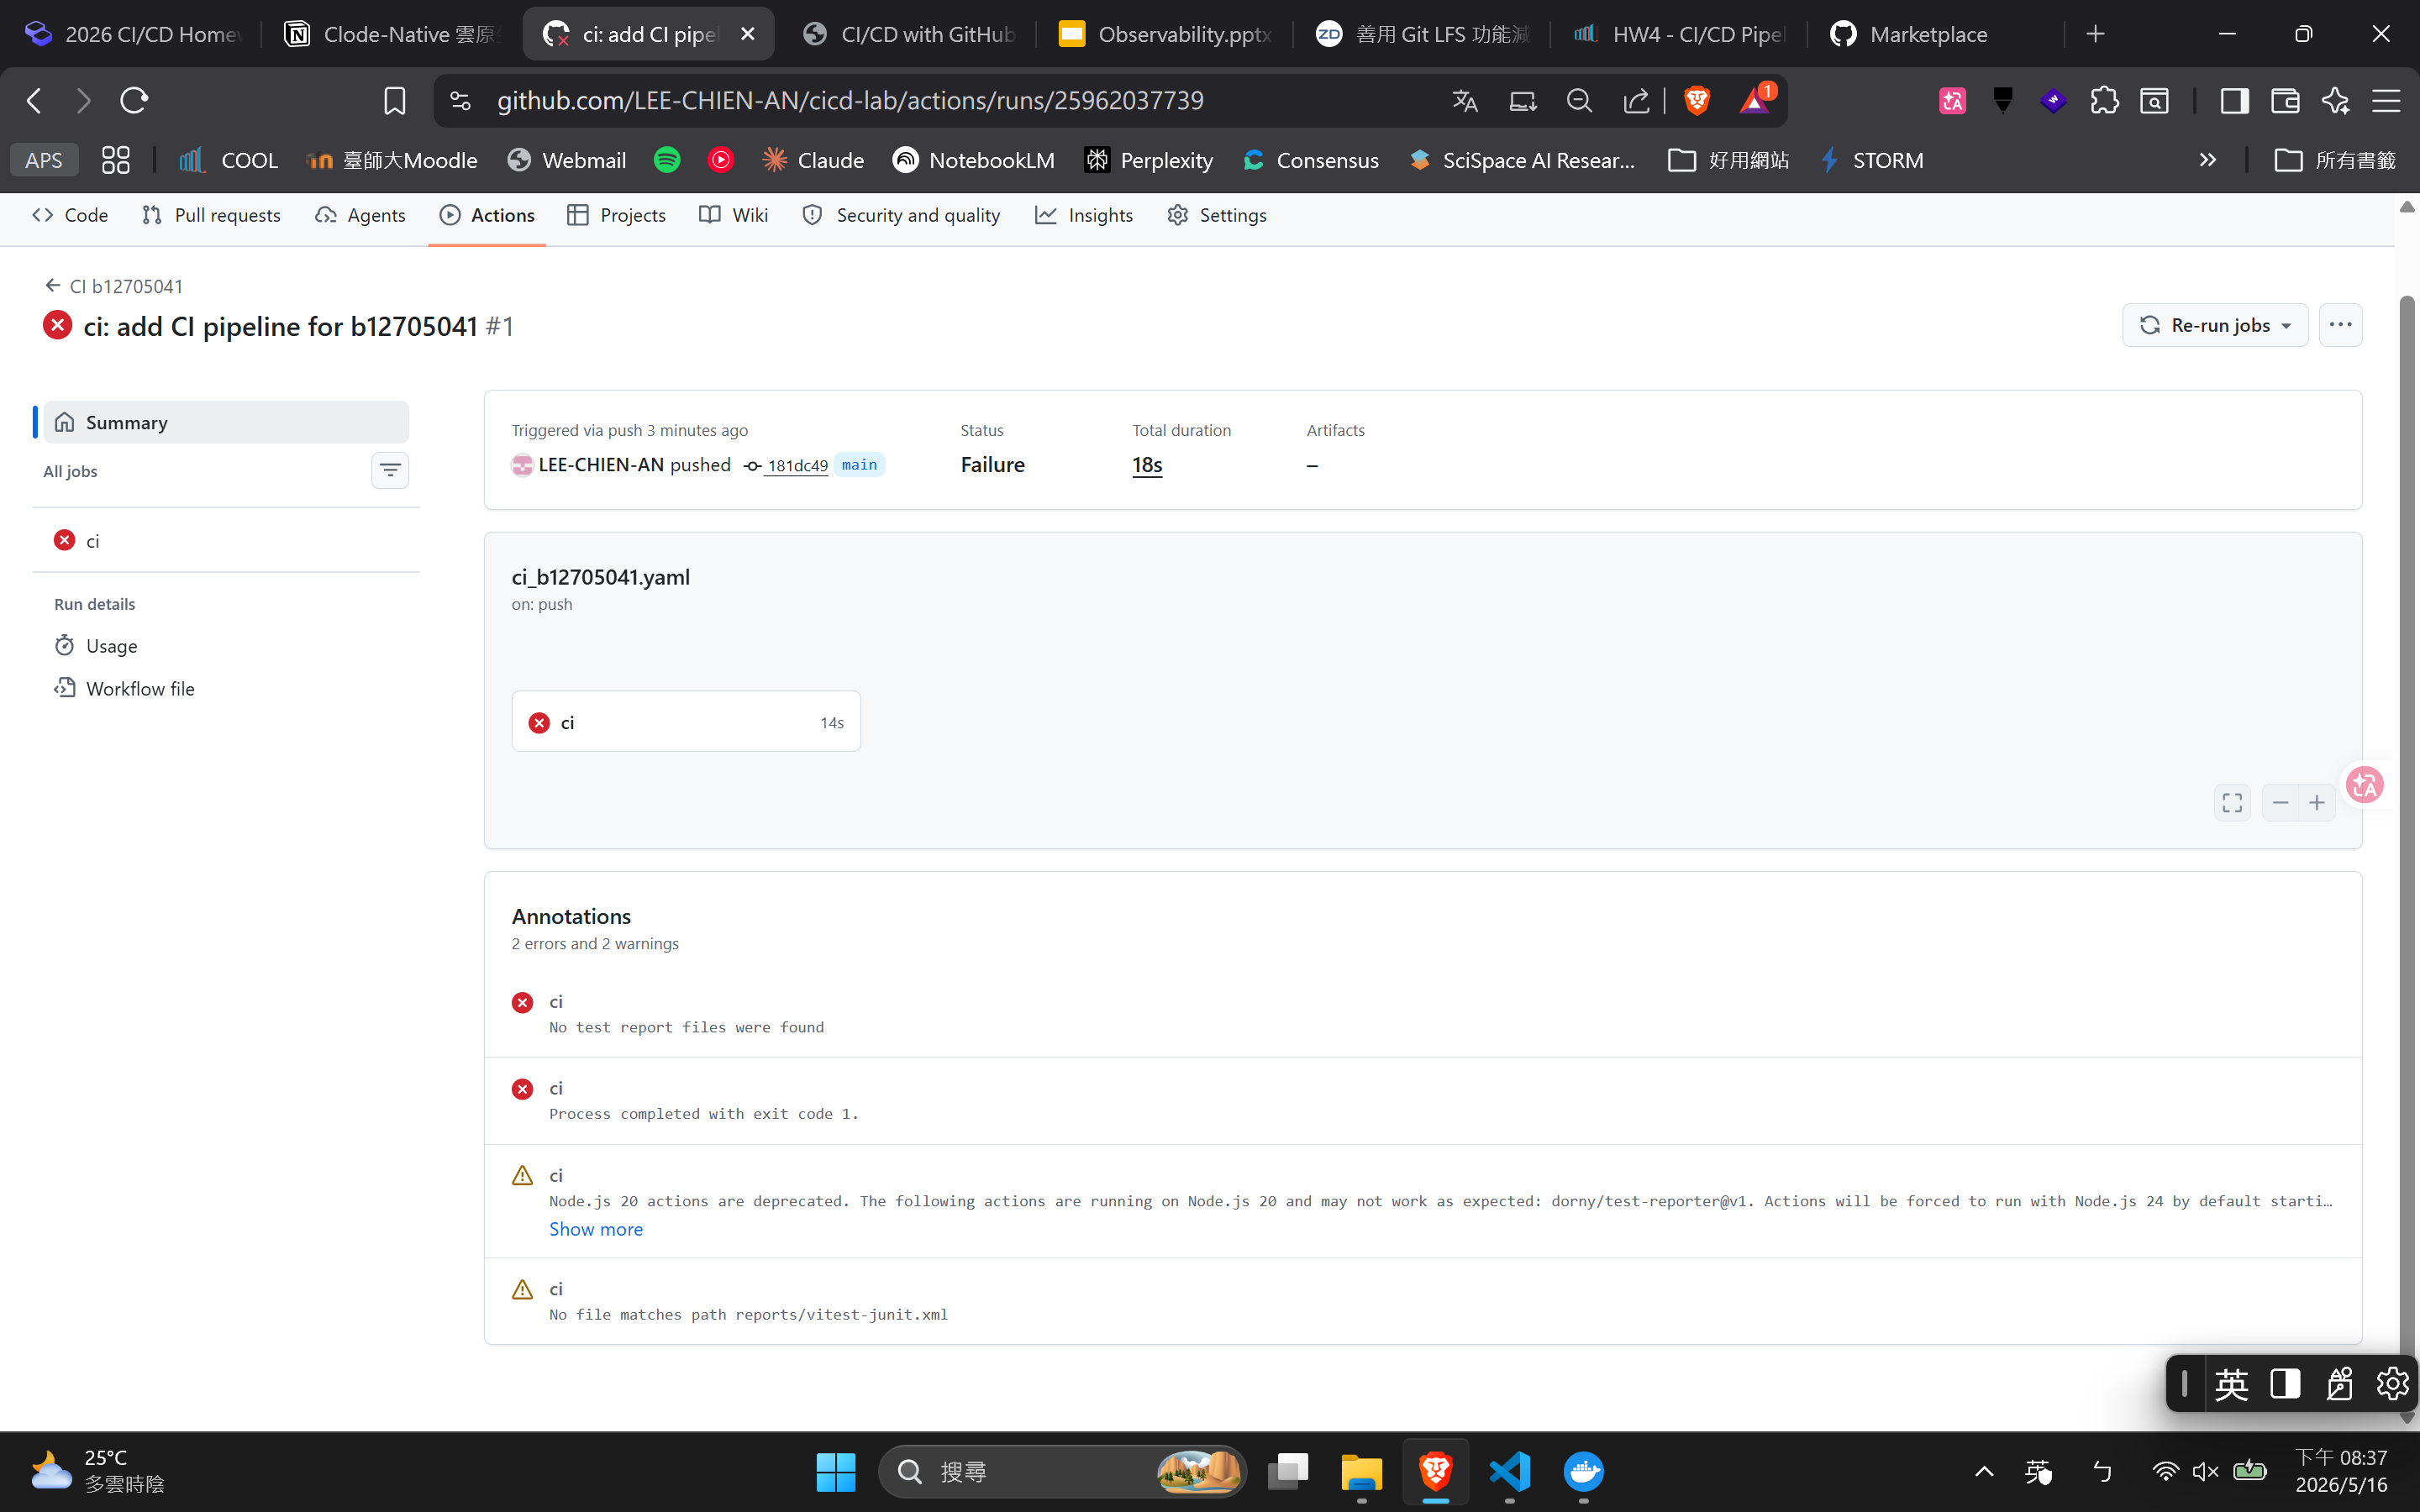
\includegraphics[width=0.8\textwidth]{image1.png}
    \caption{Prettier 格式檢查失敗，Pipeline 中止}
\end{figure}

\begin{figure}[H]
    \centering
    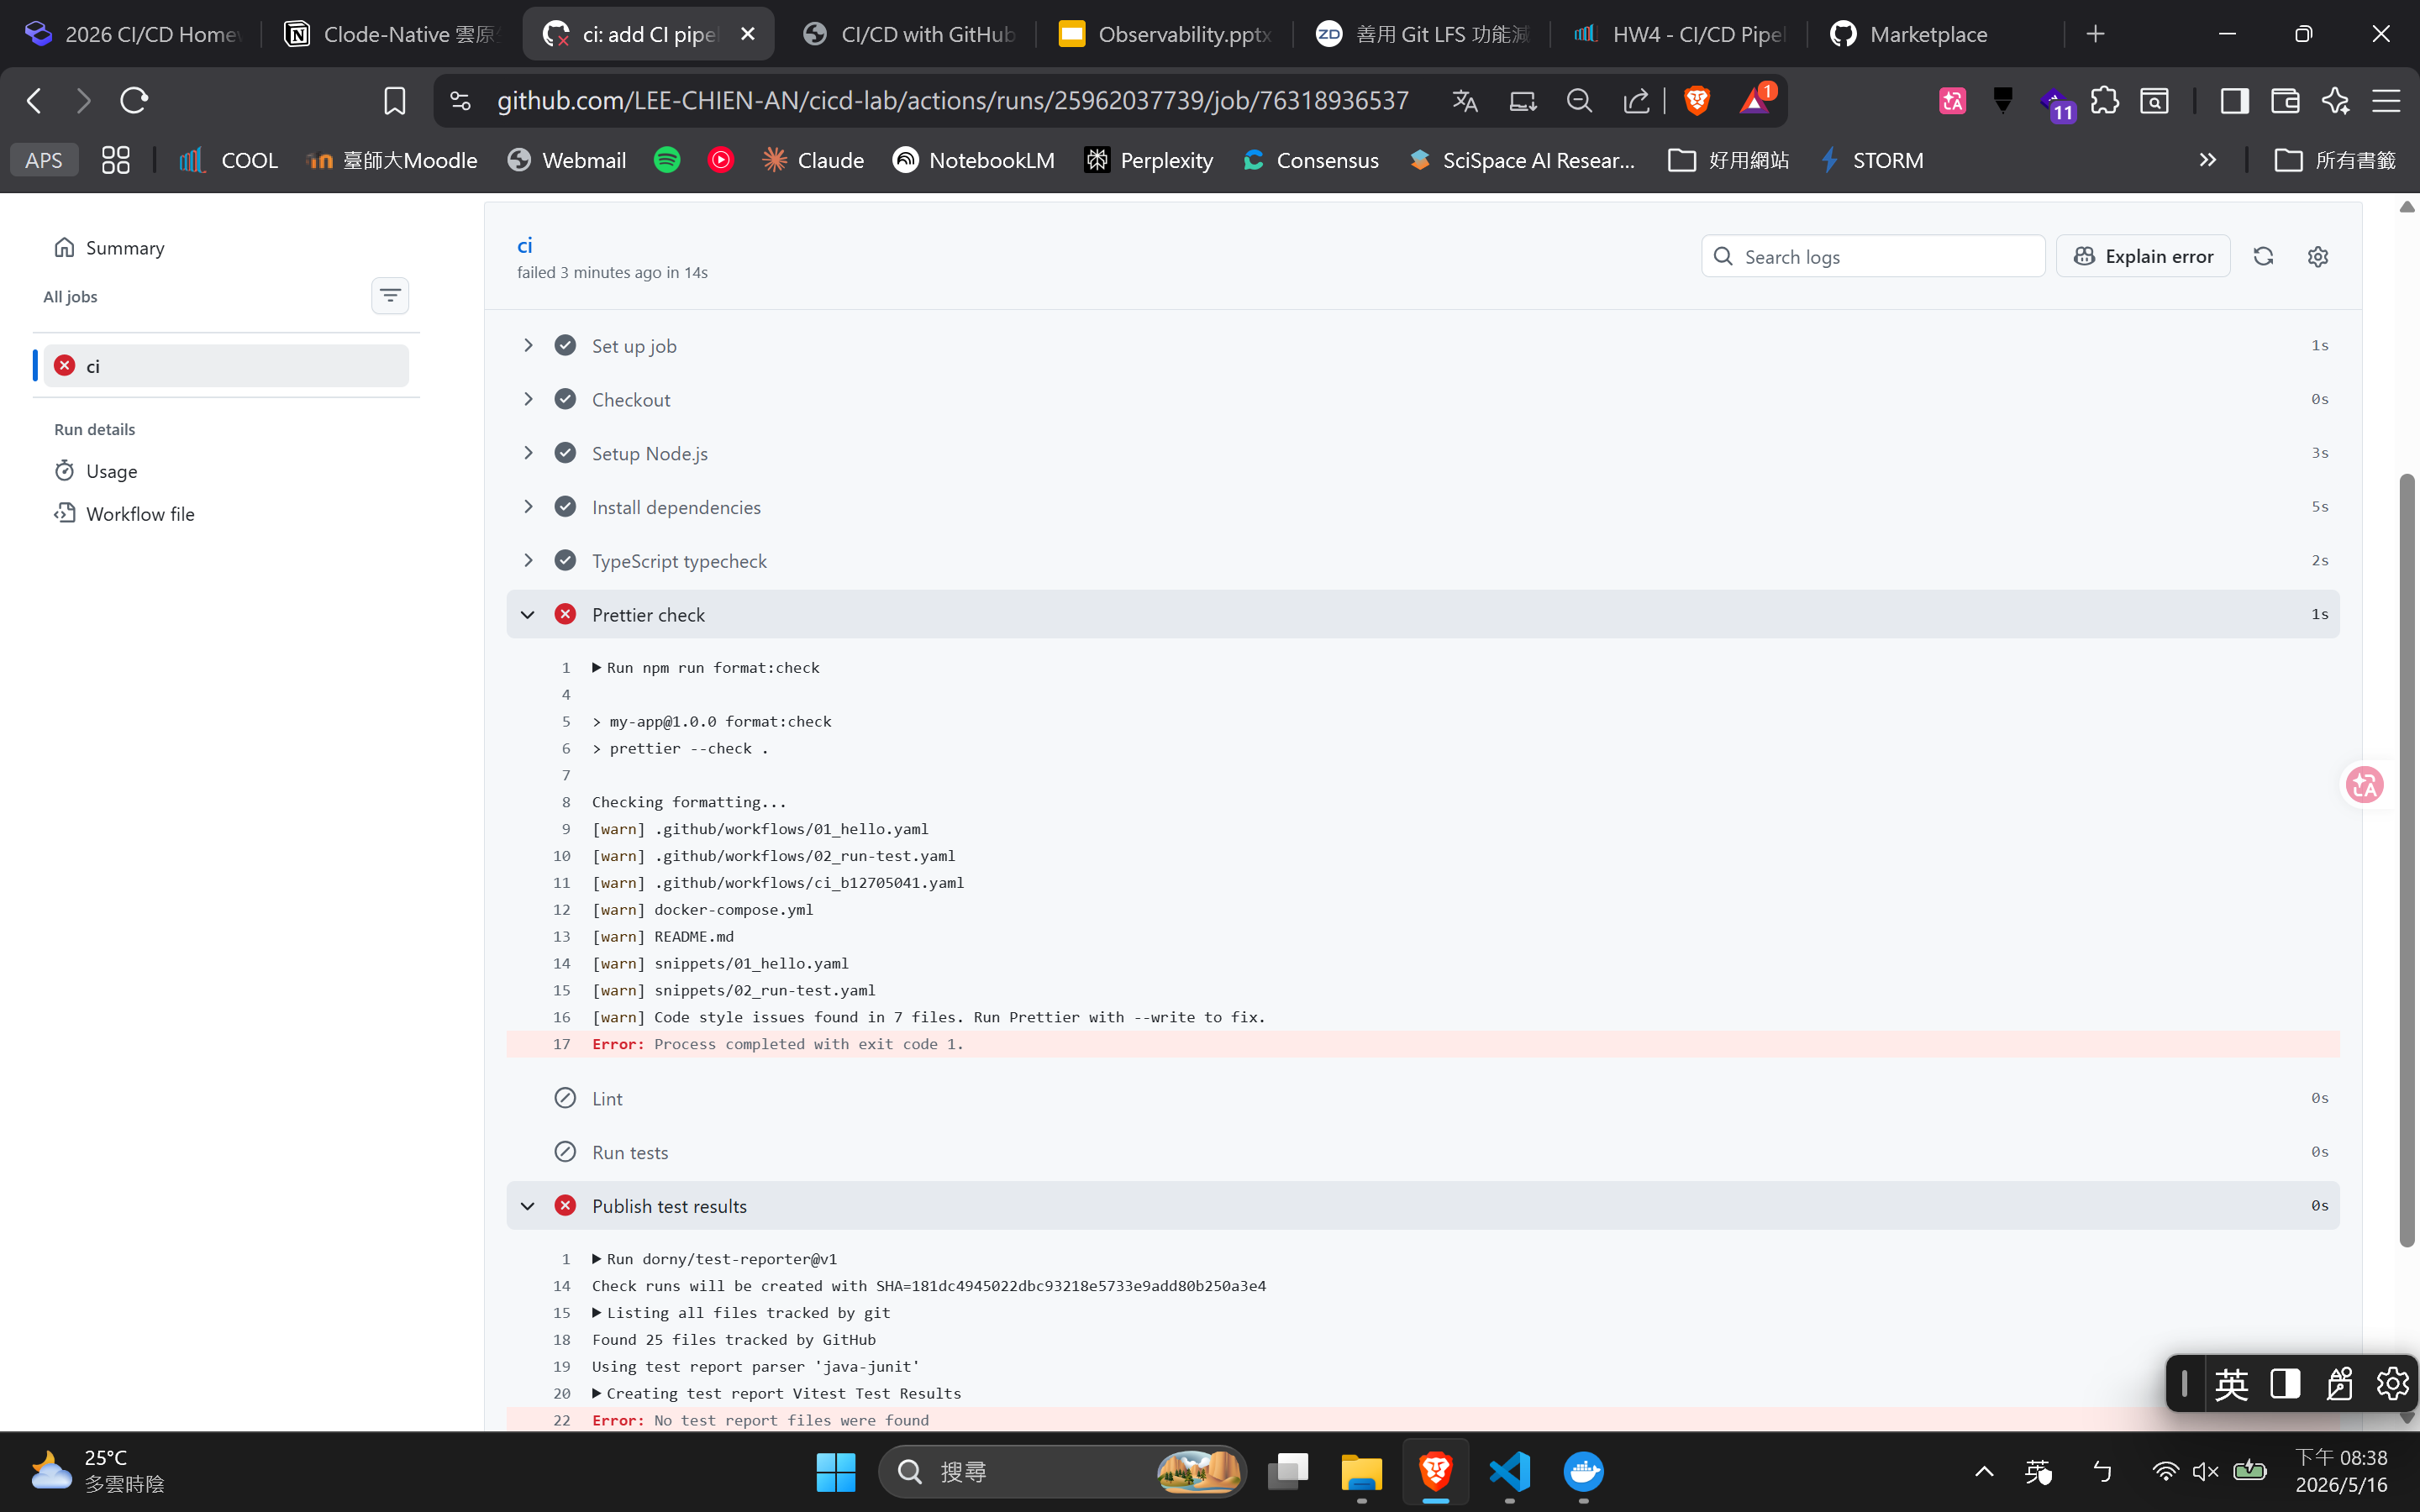
\includegraphics[width=0.8\textwidth]{image2.png}
    \caption{因測試未執行，test-reporter 找不到報告檔案}
\end{figure}

\textbf{修復方式}

執行 \texttt{npm run format}，讓 Prettier 自動修正所有格式問題後重新提交：

\begin{lstlisting}[language=Bash]
npm run format
git add -A
git commit -m "style: format all files with prettier"
git push origin main
\end{lstlisting}

\begin{figure}[H]
    \centering
    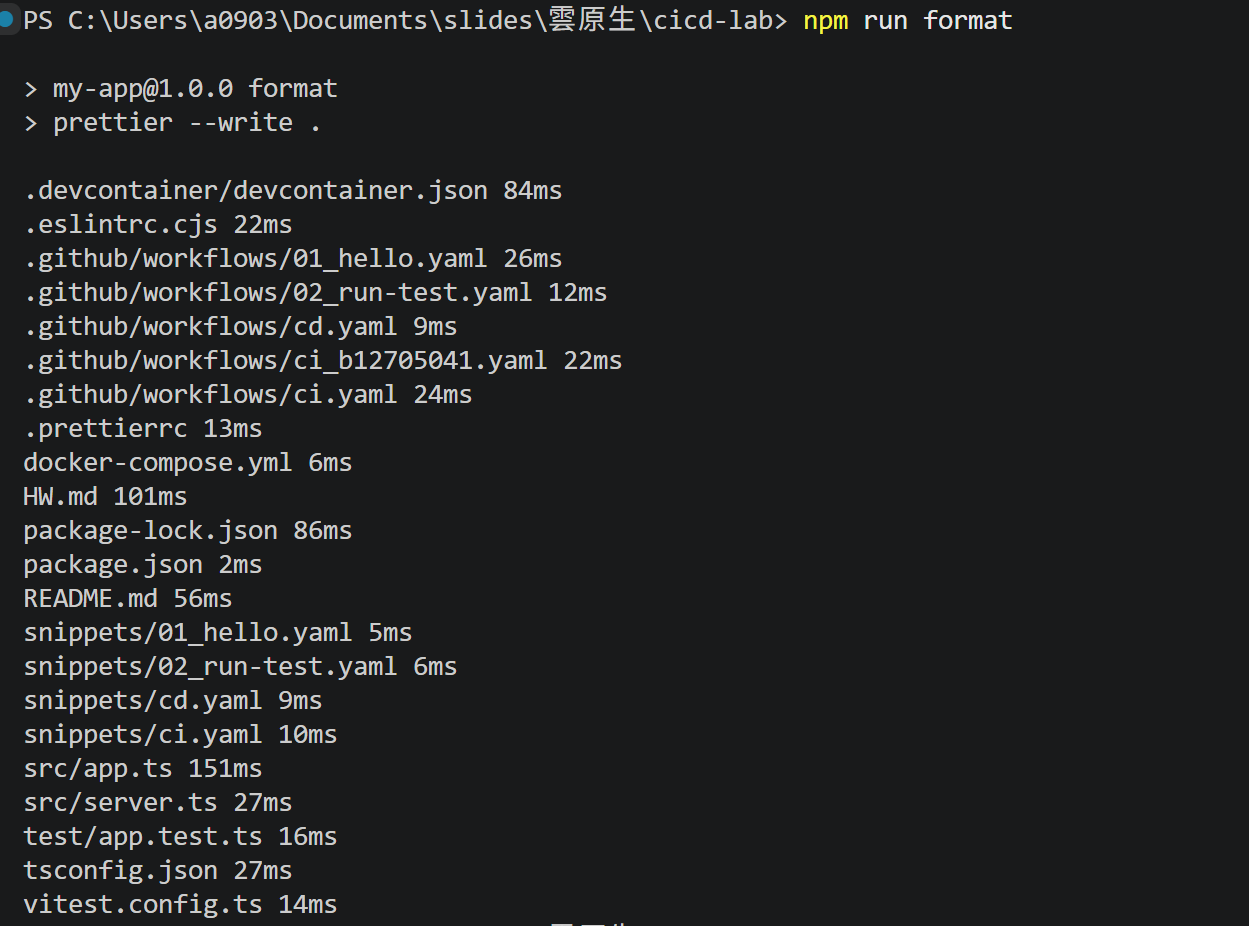
\includegraphics[width=0.7\textwidth]{image3.png}
    \caption{執行 npm run format}
\end{figure}

\subsection*{案例二：ESLint 型別感知分析失敗}

\textbf{錯誤原因}

\texttt{.eslintrc.cjs} 設定 \texttt{parserOptions.project: './tsconfig.json'}，要求 ESLint 使用 TypeScript 的型別資訊進行深度分析。然而 \texttt{tsconfig.json} 的 \texttt{include} 欄位只包含 \texttt{src/**/*.ts}，測試檔案 \texttt{test/app.test.ts} 與設定檔 \texttt{vitest.config.ts} 均不在其中，導致 ESLint 無法解析這些檔案並報錯：

\begin{lstlisting}
Parsing error: "parserOptions.project" has been set for
@typescript-eslint/parser.
The file was not found in any of the provided project(s):
test/app.test.ts
\end{lstlisting}

\begin{figure}[H]
    \centering
    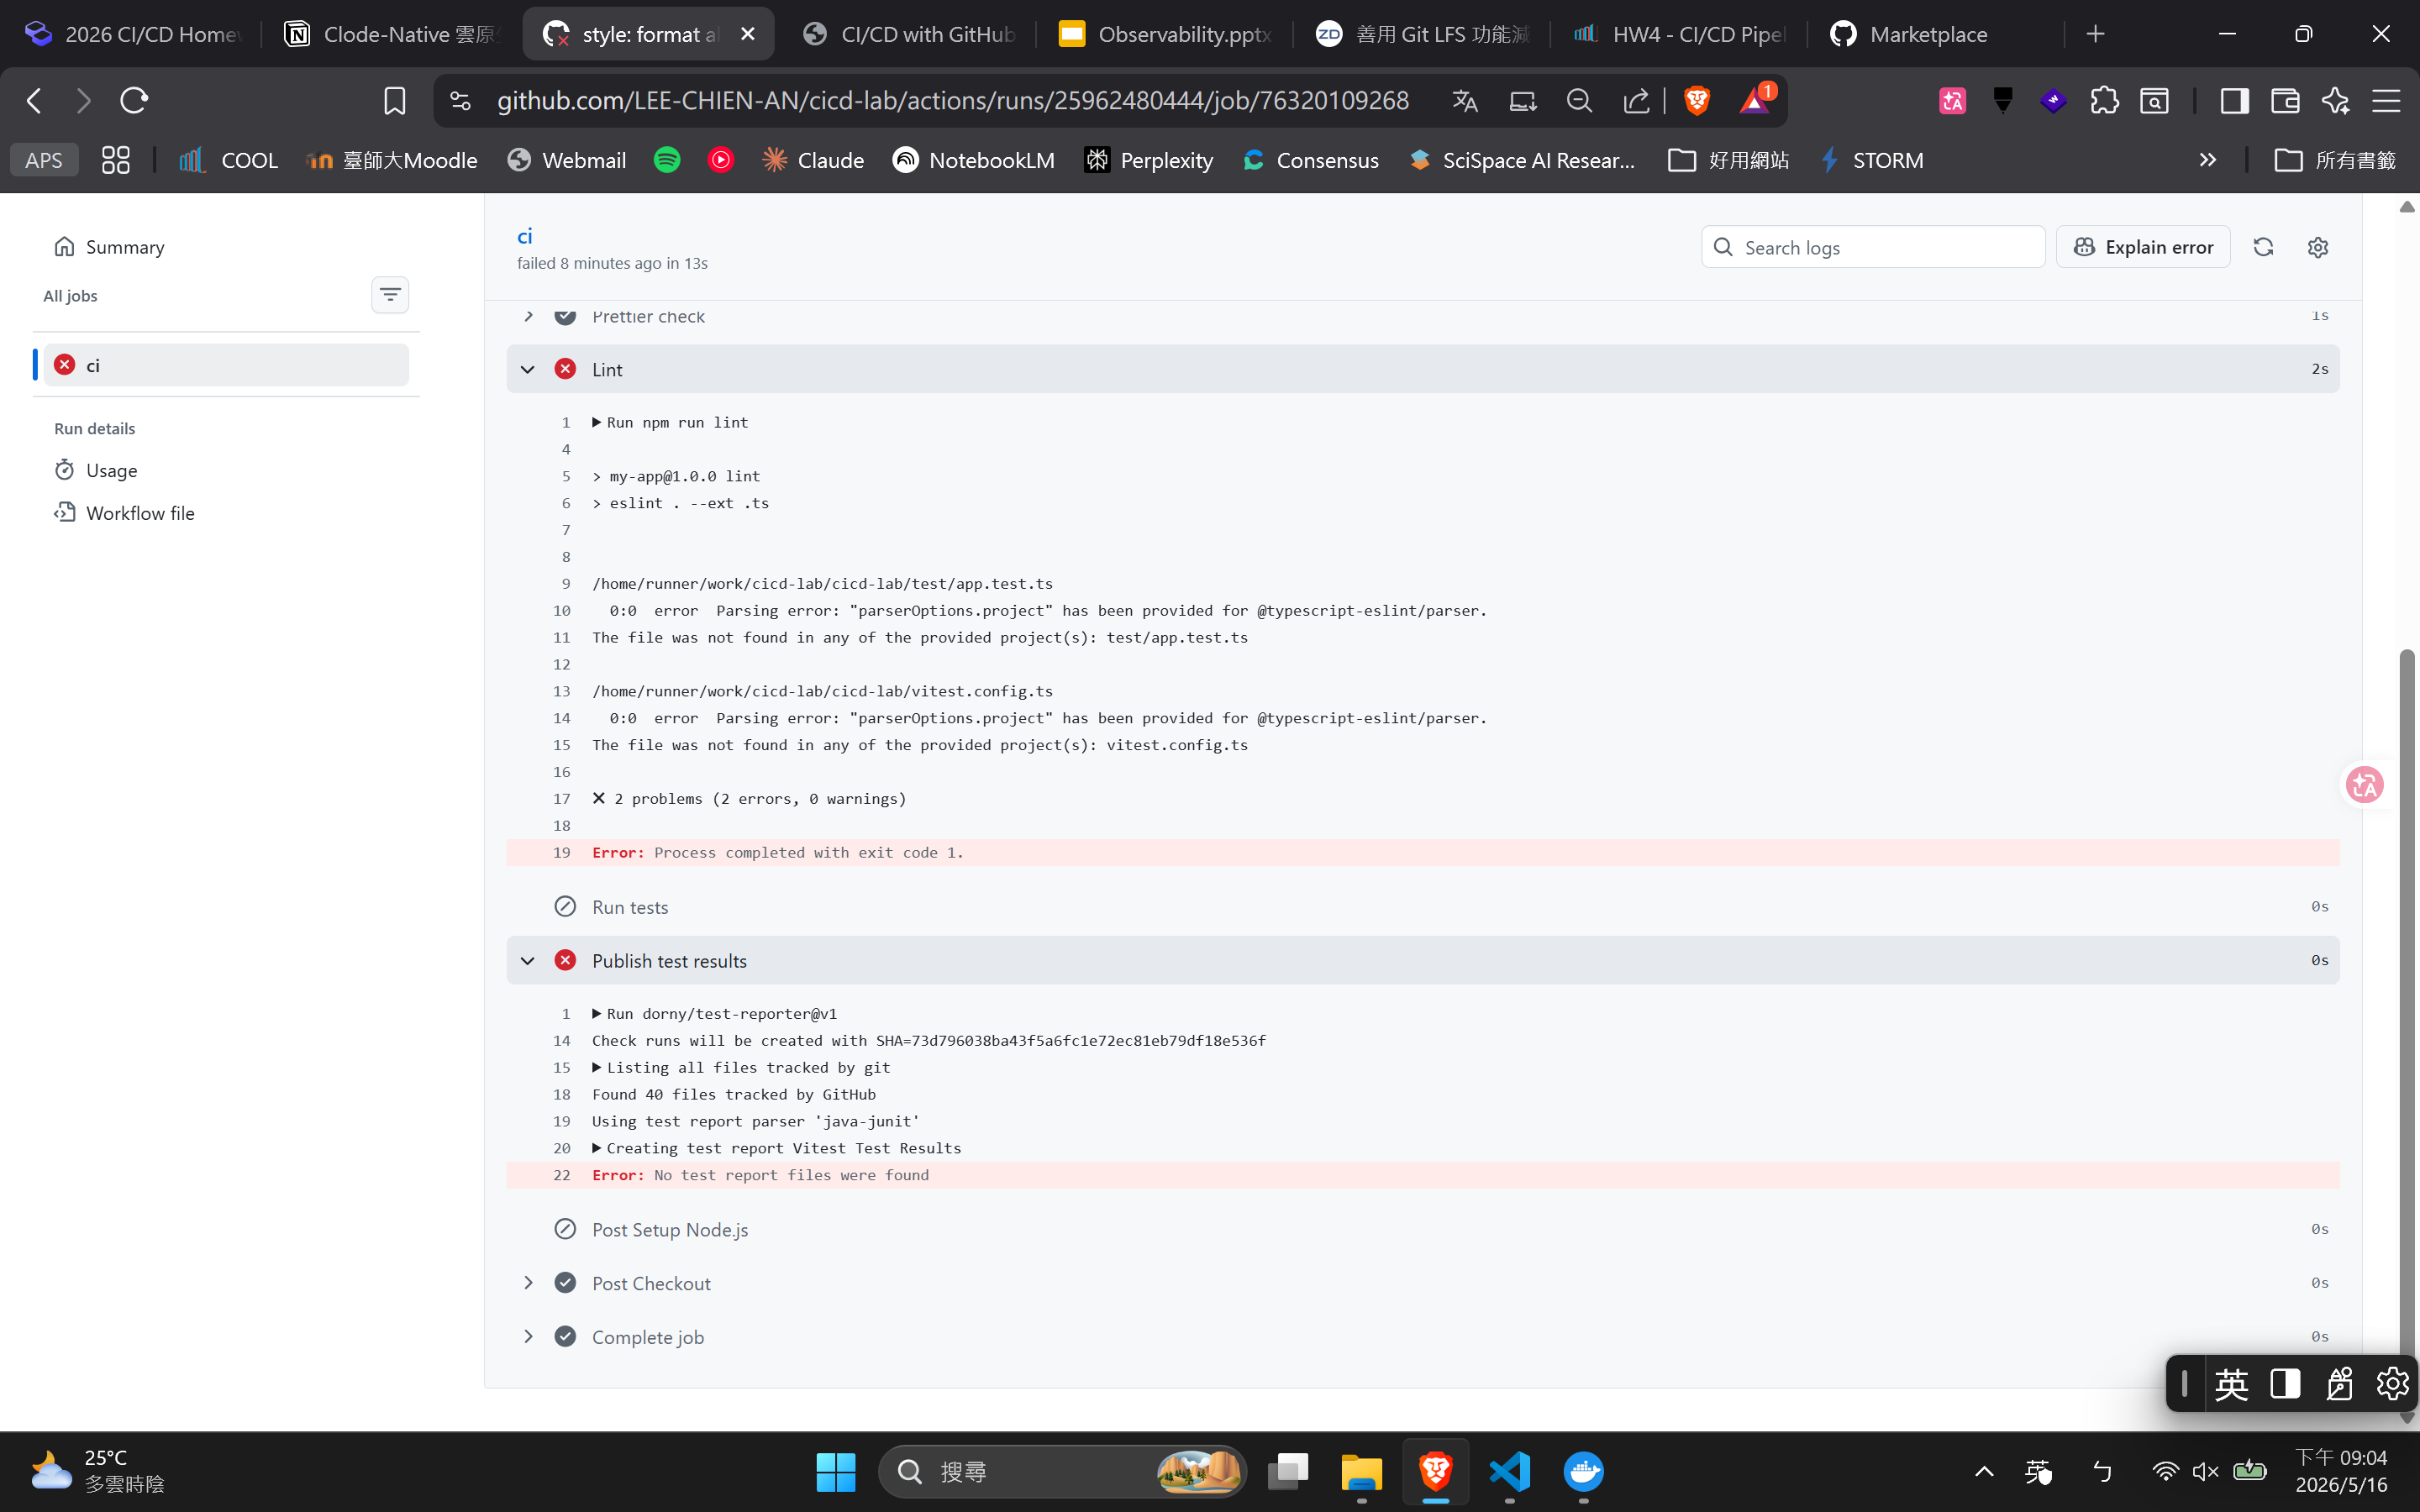
\includegraphics[width=0.8\textwidth]{image4.png}
    \caption{ESLint 因 tsconfig 設定不完整而失敗}
\end{figure}

\textbf{修復方式}

新增 \texttt{tsconfig.eslint.json}，繼承原本的 \texttt{tsconfig.json} 設定，但額外涵蓋測試檔案與設定檔，並將 \texttt{.eslintrc.cjs} 的 \texttt{project} 指向新檔案：

\begin{lstlisting}[language=YAML]
// tsconfig.eslint.json
{
  "extends": "./tsconfig.json",
  "include": ["src/**/*.ts", "test/**/*.ts", "vitest.config.ts"]
}
\end{lstlisting}

\begin{lstlisting}[language=JavaScript]
// .eslintrc.cjs (修改前後對比)
// 修改前: project: './tsconfig.json'
// 修改後: project: './tsconfig.eslint.json'
\end{lstlisting}

此做法為 \texttt{@typescript-eslint} 官方推薦的標準模式，將「Build 用的 tsconfig」與「Lint 用的 tsconfig」分離，各司其職：

\begin{table}[H]
    \centering
    \begin{tabularx}{\textwidth}{lX}
        \toprule
        \textbf{檔案} & \textbf{用途} \\
        \midrule
        \texttt{tsconfig.json} & 供 \texttt{npm run build} 使用，只需包含 \texttt{src/}，測試檔案不應進入 Production Build \\
        \texttt{tsconfig.eslint.json} & 供 ESLint 使用，在原設定基礎上額外包含 \texttt{test/} 與 \texttt{vitest.config.ts} \\
        \bottomrule
    \end{tabularx}
    \caption{tsconfig 分離策略說明}
\end{table}

\begin{figure}[H]
    \centering
    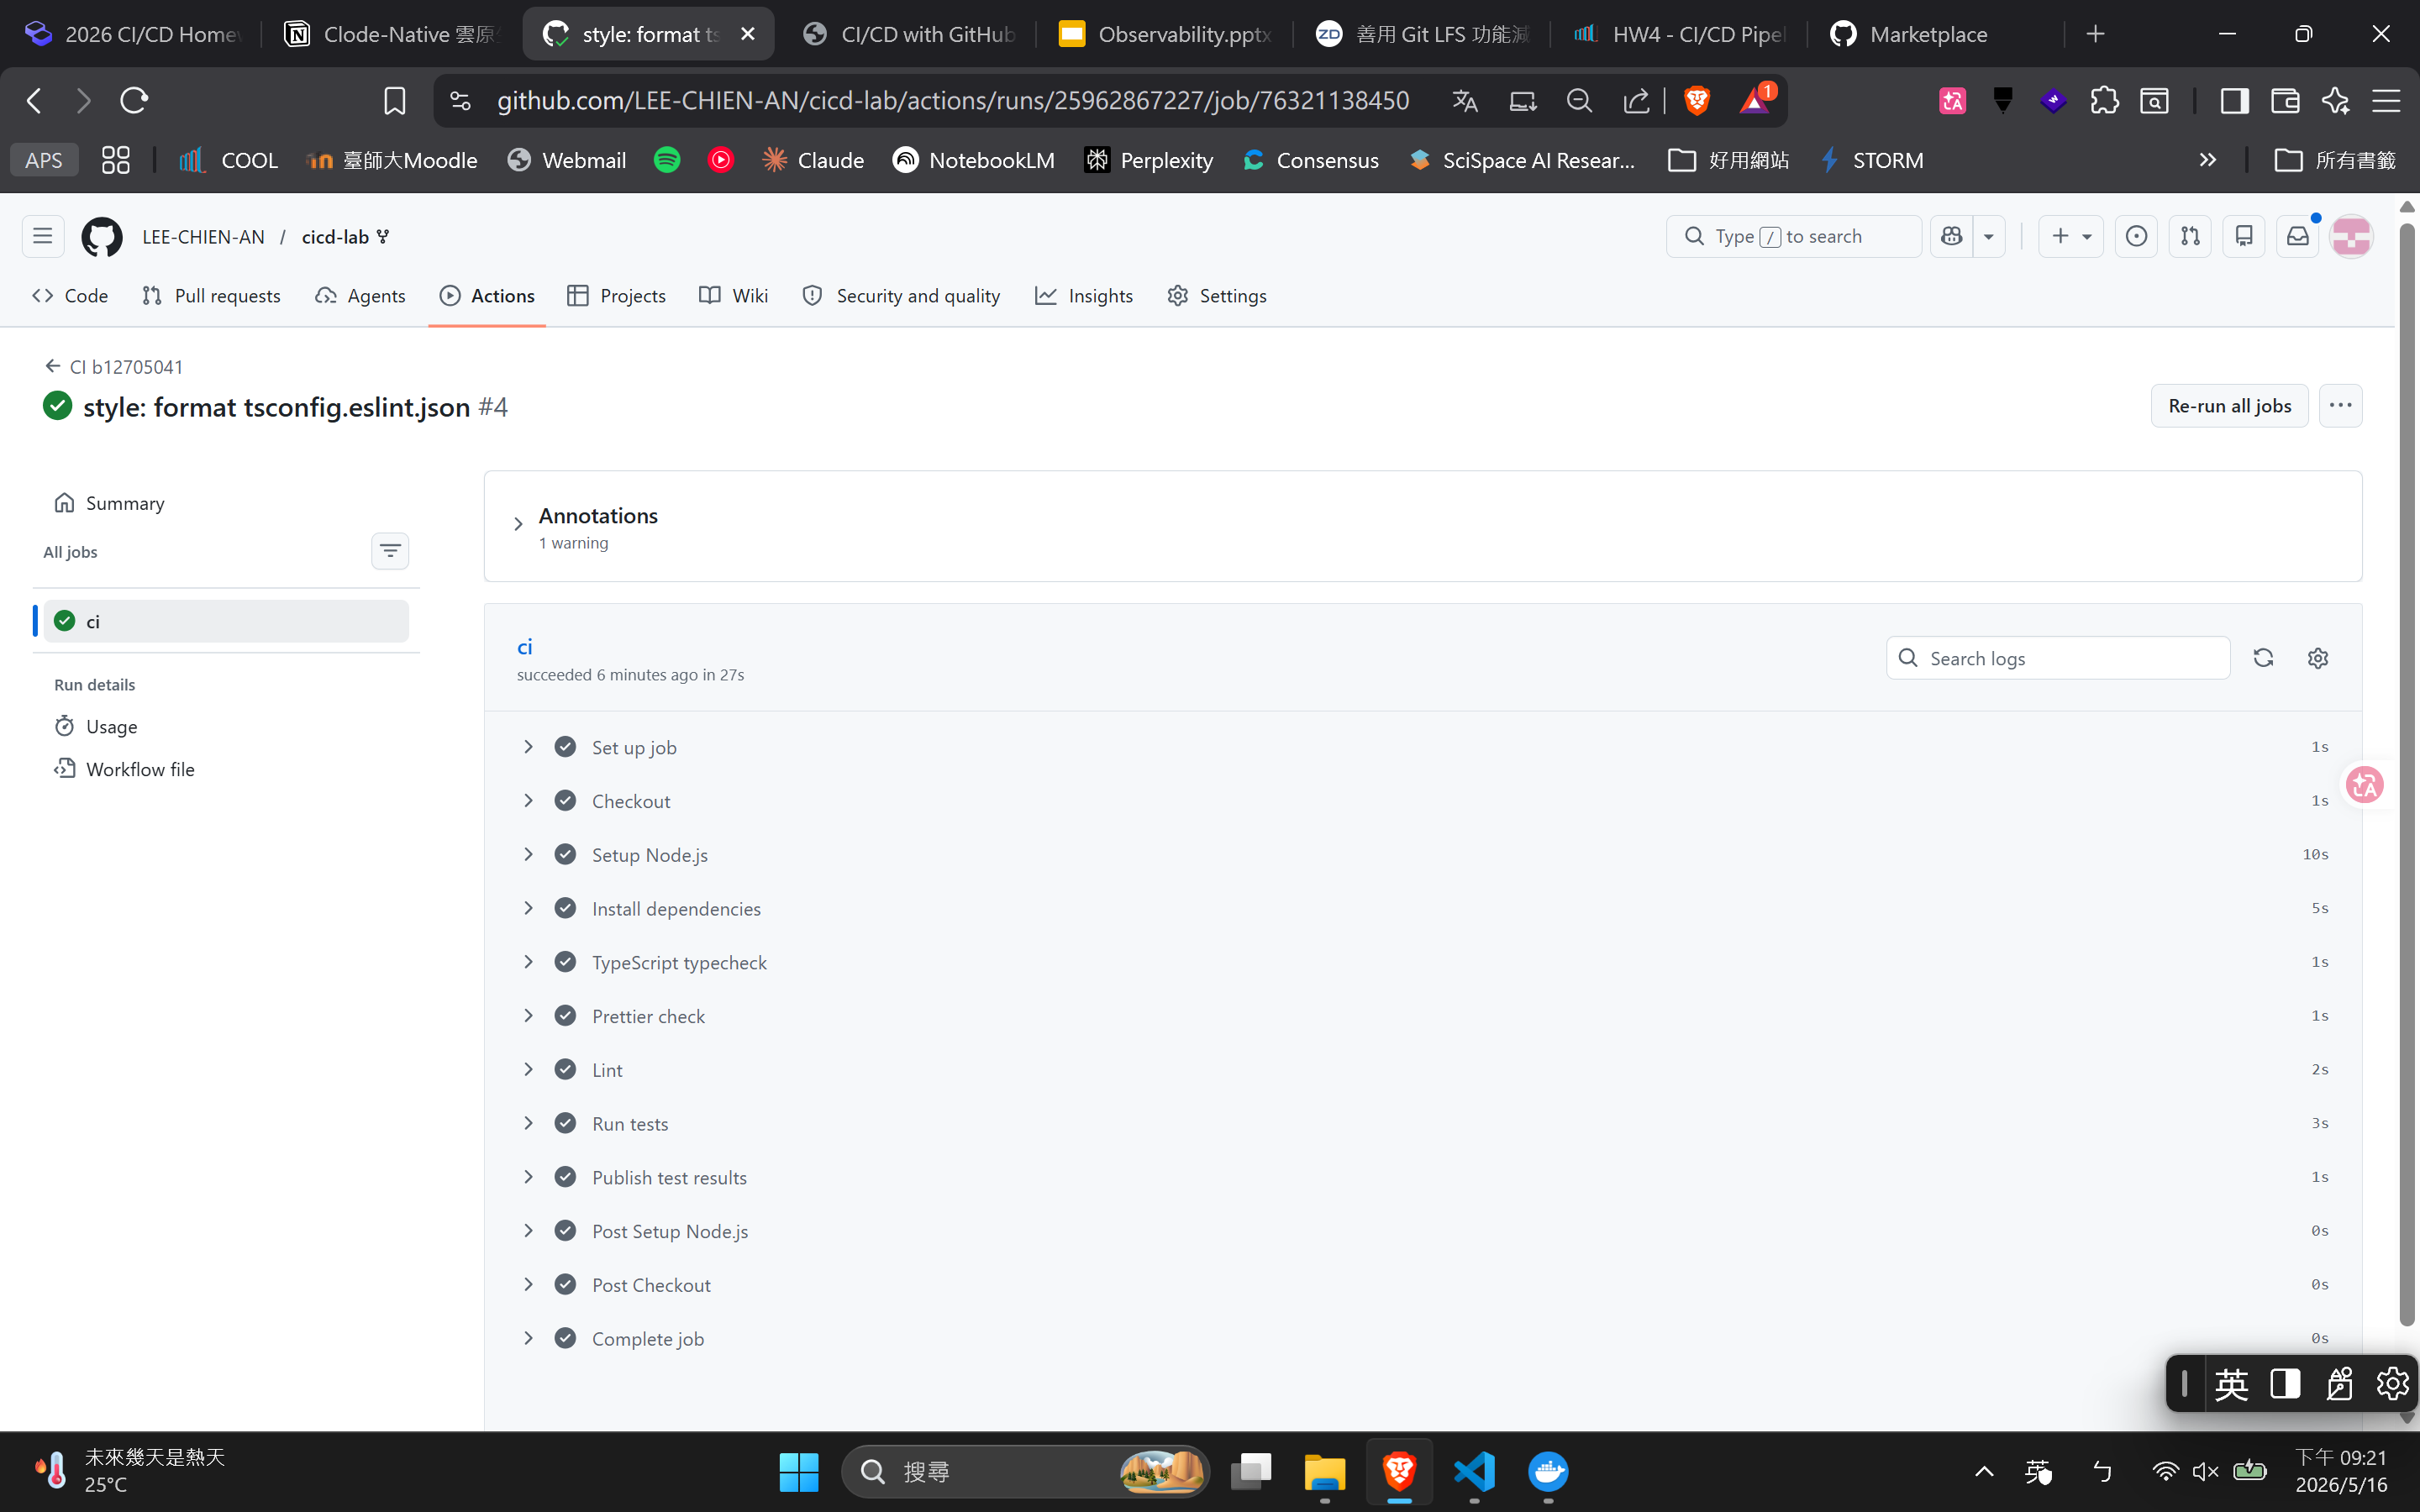
\includegraphics[width=0.8\textwidth]{image6.png}
    \caption{修復 ESLint 設定後所有步驟全數通過}
\end{figure}

\end{document}